% !TeX root = ../main.tex
\documentclass[./../main.tex]{subfiles}

\begin{document}
\section{Định dạng tệp PDF}
Tệp pdf là một trong những định dạng phổ biến nhất để lưu trữ tài liệu trên toàn thế giới. Năm 1993, PDF được Adobe Systems định nghĩa và đến năm 2008, PDF đã trở thành một tiêu chuẩn mở được phát hành dưới chuẩn ISO 32000-1.
\subsection{Các đối tượng tệp}
Cấu trúc của tệp PDF bao gồm các đối tượng liên kết với nhau trong một cấu trúc cây. Những đối tượng này được chia thành ba loại, gồm có các đối tượng đơn giản, các đối tượng ghép và đối tượng độc lập.
\begin{description}
	\item[Đối tượng đơn giản]
	      \begin{itemize}
		      \item[Boolean] lưu giá trị true/false
		      \item[Number] đối tượng số,
		      \item[String] các xâu ký tự với kích thước tối đa 65535 bytes;
		      \item[Name] là các đối tượng từ khóa được định nghĩa sẵn trong tiêu chuẩn PDF, theo sau bởi ký tự ‘/’, ví dụ ‘/kids’ xác định các đối tượng con, ‘/filter’ chỉ định bộ lọc được sử dụng,...
		      \item[Indirect reference]: là các tham chiếu tới các đối tượng độc lập.

	      \end{itemize}
	\item[Đối tượng ghép]
	      \begin{itemize}
		      \item[Array] mảng 1 chiều các đối tượng được sắp xếp trong cặp ký tự ‘[]’.
		      \item[Dictionary] giống như một danh sách lưu trữ các cặp từ khóa - giá trị, được đặt trong cặp ký tự  ‘<<>>’. Từ khóa phải là một đối tượng Name còn giá trị thì có thể là bất kể đối tượng nào. Mỗi từ khóa chỉ xuất hiện 1 lần duy nhất trong một đối tượng dictionary.
		      \item[Stream] đối tượng stream giống như một đối tượng string, gồm một chuỗi các bytes, nhưng khác ở việc không giới hạn về độ dài. Do đó đối tượng stream có khả năng chứa một lượng lớn dữ liệu như hình ảnh, các thông tin mô tả trang,... Stream được đặt trong cặp từ khóa ‘stream endstream’.
	      \end{itemize}
	\item[Đối tượng độc lập]
	      Các đối tượng độc lập có định danh là các cặp (number object, generation object) ứng với số thứ tự đối tượng và thế hệ của đối tượng. Các đối tượng khác có thể tham chiếu tới qua định danh này. Các đối tượng độc lập được định nghĩa bên trong cặp từ khóa ‘obj endobj’.

\end{description}


\subsection{Cấu trúc vật lý}
Cấu trúc vật lý của PDF xác định cách đối tượng được lưu trữ trong tệp, cách mà chúng được truy cập và cập nhật.
Một tệp PDF cơ bản sẽ được xây dựng bằng bốn yếu tố: header, body, bảng tham chiếu xref table và trailer. Hình \ref{fig:initstruct} thể hiện cấu trúc này.
Cấu trúc ban đầu của PDF sẽ được thay đổi sau mỗi lần cập nhật, bằng cách thêm các sự thay đổi vào cuối của tệp, được gọi là cập nhật tăng dần.
% figure
\begin{figure}[ht!]
	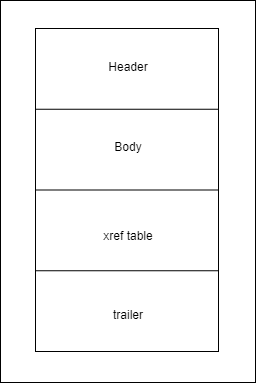
\includegraphics[width=\linewidth]{./images/initial_structure.png}
	\caption{Cấu trúc vật lý của tệp PDF}
	\label{fig:initstruct}
\end{figure}

\begin{description}
	\item[Header]
	      Header là dòng đầu tiên trong tệp PDF, xác định phiên bản tệp, được viết dưới định dạng ‘%PDF-version’. Ví dụ ‘%PDF-1.7’ xác định phiên bản PDF hiện tại là 1.7.
	      Ngoài ra, nếu tệp PDF chứa dữ liệu nhị phân, header sẽ chứa một dòng comment gồm ít nhất 4 ký tự nhị phân giúp xác định được cần xử lý dữ liệu tệp dưới dạng văn bản hay nhị phân.

	\item[Body]
	      Phần body của tệp chứa tất cả các đối tượng lưu trữ những dữ liệu sẽ hiển thị cho người dùng, được xác định từ sau phần header đến khi xuất hiện từ khóa ‘xref’. Những dữ liệu trong body sau đó có thể được chỉnh sửa, và phần cập nhật sẽ được lưu trữ ở cuối tệp.
	\item[Xref Table]
	      Xref table hay còn được gọi là cross-reference table là một bảng tham chiếu tới các đối tượng độc lập trong tài liệu nhằm mục đích cho phép truy cập ngẫu nhiên vào các đối tượng này mà không cần đọc toàn bộ tài liệu để định vị một đối tượng cụ thể.
	      Bảng có thể chứa 1 hoặc nhiều phần. Ban đầu, toàn bộ bảng chỉ bao gồm 1 phần duy nhất. Một phần tương ứng sẽ được thêm vào nếu tệp được thay đổi.
	      % figure
	      \begin{figure}[ht!]
		      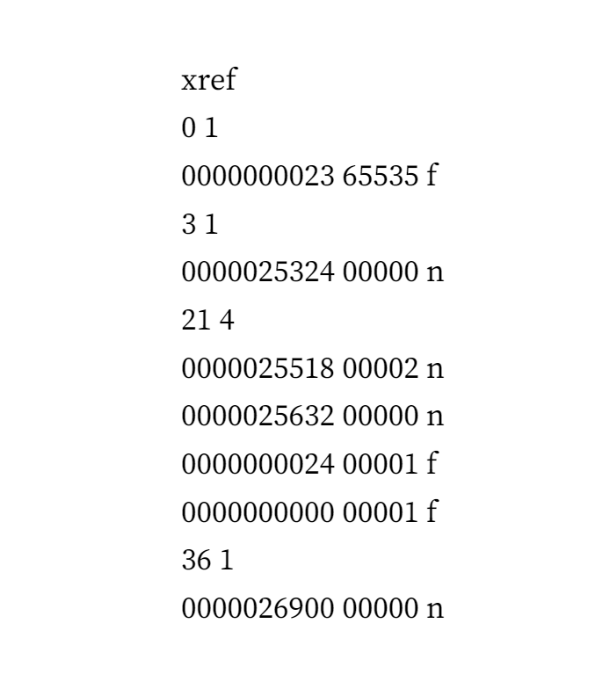
\includegraphics[width=\linewidth]{./images/xref_example.png}
		      \caption{Một bảng xref trong tài liệu PDF}
		      \label{fig:xreftable}
	      \end{figure}


	      Ở trên hình \ref{fig:xreftable}, cho thấy một ví dụ về bảng tham chiếu trong tệp PDF, gồm có 4 phần con, bắt đầu bởi dòng chứa hai giá trị số với giá trị đầu là số thứ tự của đối tượng đầu tiên, giá trị thứ hai là số lượng đối tượng trong phần con này. Ví dụ ở phần thứ 3, giá trị ‘21 4’ cho thấy có 4 đối tượng trong phần con, được đánh số bắt đầu từ 21 đến 24. Theo sau đó là các dòng đại diện cho các đối tượng, xác định bởi một chuỗi gồm 20 byte lưu trữ địa chỉ của đối tượng (offset), số thế hệ của đối tượng và một cờ ‘f’ hoặc ‘n. Cờ ‘f’ nghĩa là đối tượng vẫn tồn tại trong tệp nhưng được đánh dấu không nên được sử dụng, ngược lại, cờ ‘n’ xác định đối tượng đang được sử dụng.
	\item[Trailer]

	      Trailer PDF được lưu ở cuối tệp, chỉ định vị trí của bảng tham chiếu và các đối tượng đặc biệt khác, bắt đầu bởi từ khóa ‘trailer’ \ref{fig:trailer}.

	      % figure
	      \begin{figure}[ht!]
		      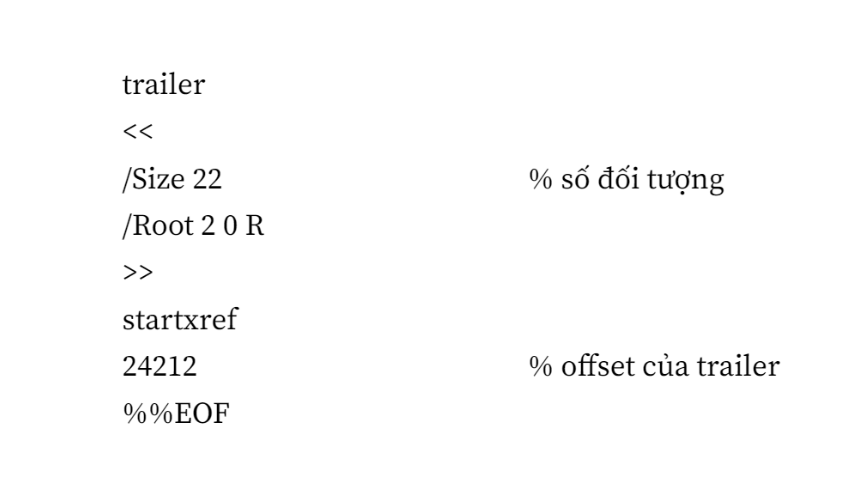
\includegraphics[width=\linewidth]{./images/img_trailer_pdf.png}
		      \caption{Một trailer trong tài liệu PDF}
		      \label{fig:trailer}
	      \end{figure}

	      Trong đối tượng dictionary của trailer lưu trữ các giá trị:

	      \begin{itemize}
		      \item[Size] xác định số lượng đối tượng trong bảng tham chiếu (có đếm cả các đối tượng trong các phần mới cập nhật). Giá trị này phải là 1 số nguyên, và không thể là một đối tượng tham chiếu.
		      \item[Prev] xác định địa chỉ của bảng tham chiếu được cập nhật trước đó- được sử dụng khi có nhiều bảng tham chiếu.
		      \item[Root] tham chiếu tới một đối tượng gốc trong mô hình cấu trúc logic của PDF.
	      \end{itemize}

\end{description}
\end{document}
\subsection{Cấu trúc logic}

\section{Một số thuật toán phân loại}

\section{Phát hiện tài liệu PDF độc hại}



\end{document}